
\begin{frame}
\frametitle{Outline} 
\tableofcontents[currentsection]
\end{frame}

\begin{frame}
\frametitle{Gradual typing: no big-bang migration}
\textbf{\color{darkslateblue}Two non-negotiable requirements for real-world adoption by existing languages:}\\
\textbf{\hspace*{.4mm}1.} You do not have to type-annotate your entire codebase at once.\\
\textbf{2.} Types do not modify the run-time semantics of existing programs.

\medskip

\begin{block}{The \code{dynamic()} type}
\begin{itemize}
\setlength{\itemsep}{-0pt}
\item May turn into any other type at runtime: typed and untyped code coexist
      seamlessly
\item Offers a more relaxed type safety guarantee:\\
 If some program \code{e} has type \code{integer()} and evaluates to a value, \\
      then this value is of type \code{integer()}.
\end{itemize}
\end{block}

\end{frame}
%%% def boolean_id(x), do: x
\defverbatim[colored]{\weakApp}{
\begin{minted}{elixir}
id_weak(x_dyn)                    !\textcolor{gray}{\footnotesize x\textunderscore{}dyn may be a string, and}!
# type dynamic()                  !\textcolor{gray}{\footnotesize id\textunderscore{}weak returns it unchanged}!
\end{minted}
}
\defverbatim[colored]{\strongApp}{
\begin{minted}{elixir}
id_weak(x_dyn)                    id_strong(x_dyn)
# type dynamic()                  # type integer() 
\end{minted}
}
\defverbatim[colored]{\strongAppPropagation}{
\begin{minted}{elixir}
id_weak(x_dyn)                    id_strong(x_dyn)
# type dynamic()                  # type integer() !\color{magenta}and dynamic()!
\end{minted}
}

\begin{frame}
\frametitle{The gradual typing conundrum}
\textbf{\color{darkslateblue}Typing every expression by \code{dynamic()} is trivially sound \ldots but hardly useful.}

\bigskip
\pause
The system must fulfill two opposite requirements
\begin{enumerate}
	\item it must use \code{dynamic()}  as little as possible so as to be useful, and
	\item it must use \code{dynamic()} enough so as not to hinder the versatility of
	      gradual typing
\end{enumerate}


\bigskip
\pause
The first requirement is fulfilled by the typing of \textbf{\color{darkslateblue}strong functions}, which leverage the run-time checks written by the programmer, or performed by the VM\\[3mm]
The second requirement is fulfilled by the \textbf{\color{darkslateblue}propagation of \code{dynamic()}}.
\end{frame}

\subsection{Strong function types}

\begin{frame}[fragile]{Strong function types}\transdissolve<2,4->
\vspace{-1.5mm}
\begin{block}{(Weak) function type}
\begin{minted}[escapeinside=!!]{elixir}
!\spec! integer() -> integer()
def id_weak(x), do: x !\label{c1}!
\end{minted}
\end{block}
\vspace{-1.6mm}
\pause
\begin{block}{Let \code{x_dyn} be of type \code{dynamic()}}
\vspace{-4.9mm}
    \begin{overlayarea}{\textwidth}{1.3cm}
        \only<2-3>{\weakApp}
        \only<4-7>{\strongApp}
        \only<8->{\strongAppPropagation}
   \end{overlayarea}
\end{block}
\vspace{-1.5mm}
\pause
\begin{block}{Strong function type \only<6->{\smash{(by the programmer)}}}
\begin{minted}[linenos=false,escapeinside=!!]{elixir}
!\spec! integer() -> integer()
def id_strong(x) when is_integer(x), do: x 
\end{minted}
\end{block}
% \begin{block}{Application}
% \begin{minted}{elixir}
% !\spec! dynamic() -> {dynamic(), integer()}
% def dynamic_fun(x), do: {id_weak(x), id_strong(x)}
% \end{minted}
% \end{block}
\pause\pause\pause\pause
\vspace{-.5mm}
% \frametitle{Strong function types (by the VM)}
\begin{block}{Strong function type (by the VM)}
\begin{minted}[linenos=false,escapeinside=!!]{elixir}
!\spec! number() -> number()
def double(x), do: x + x
\end{minted}
\end{block}
% \begin{itemize}
% \item Functions with strong types guarantee correct output or runtime type-check failure
% \item Ensures stronger type safety guarantee without modifying Elixir compilation
% % \item Take into account user type checks
% % \item Allows for propagation of \code{dynamic()} type in certain cases
% \end{itemize}
\only<5,6>{\begin{textblock}{15}(1.3,12.9)
    \textbf{\color{darkslateblue}\large Strong function: on \emph{any} argument, even outside its domain, it returns a result in its codomain or fails}
\end{textblock}}
\only<9>{\begin{textblock}{5}(0,0)
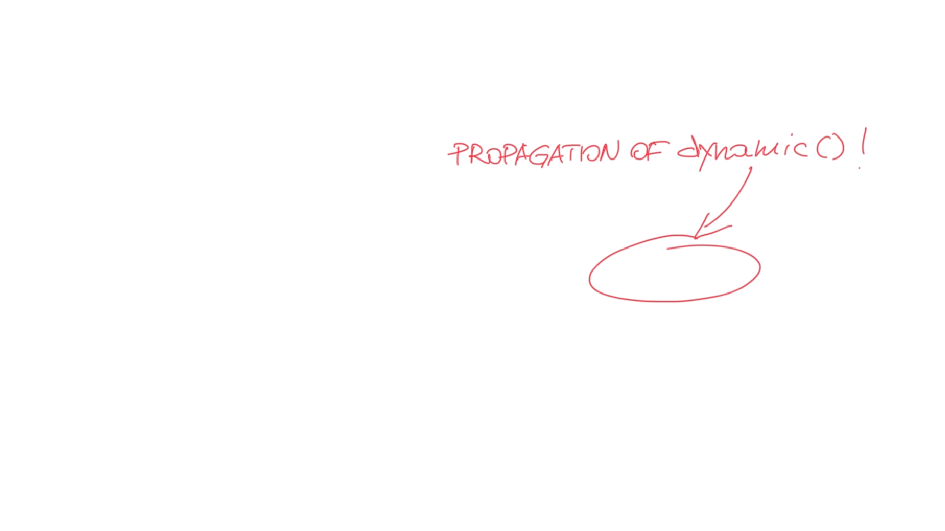
\includegraphics[scale=1]{images/hw-dynprop.pdf}
\end{textblock}}
\end{frame}




\defverbatim[colored]{\dynType}{
\begin{minted}{elixir}
#=> negate(x_dyn): (integer() or boolean()) !\color{magenta}and dynamic()!
\end{minted}
}
\defverbatim[colored]{\wrongType}{
\begin{minted}{elixir}
#=> negate(x_dyn): (integer() or boolean())
\end{minted}
}
\defverbatim[colored]{\typeError}{
\begin{minted}{elixir}
#=> Without propagation: type error, + undefined for booleans
\end{minted}
}
\defverbatim[colored]{\goodType}{
\begin{minted}{elixir}
#=> subtract: (dynamic(), dynamic() -> number())
\end{minted}
}
\defverbatim[colored]{\betterType}{
\begin{minted}{elixir}
#=> subtract: (dynamic(), dynamic() -> number() !\color{magenta}and dynamic()!)
\end{minted}
}
\defverbatim[colored]{\subtract}{
\begin{minted}{elixir}
def subtract(a, b), do: a + negate(b)
\end{minted}
}
\defverbatim[colored]{\subtractann}{
\begin{minted}{elixir}
def subtract(a, b), do: a + negate(b)    !\textcolor{gray}{\footnotesize\char35{} a, b not annotated, hence dynamic()}!
\end{minted}
}

\subsection{Propagation of \texttt{dynamic()}}

\begin{frame}[fragile]{Propagation of \texttt{dynamic()}}\transdissolve<6>
\textbf{\color{darkslateblue}Apply the (strong function) \code{negate()} function to a \code{dynamic()} argument: \code{x_dyn}}
\vspace{-4mm}
\begin{block}{\vspace{-5mm}}
\begin{minted}{elixir}
!\spec! (integer() -> integer()) and (boolean() -> boolean())
def negate(x) when is_integer(x), do: -x
def negate(x) when is_boolean(x), do: not x
\end{minted}
\vspace{-6.1mm}
\begin{overlayarea}{\textwidth}{2mm}
    \only<2-5>{\wrongType}
    \only<6->{\dynType}
\end{overlayarea}
\hfill
\vspace{0.5mm}
\hfill
\end{block}
\pause\pause\vspace{-6mm}
\begin{block}{\vspace{-6mm}}\vspace{-2mm}
\begin{overlayarea}{\textwidth}{9mm}
\only<3>{\subtract}
\only<4->{\subtractann}
\end{overlayarea}
\vspace{-6.5mm}
\begin{overlayarea}{\textwidth}{2mm}
    \only<5>{\typeError}
    \only<7>{\goodType}
    \only<8->{\betterType}
\end{overlayarea}
\hfill
\vspace{0.5mm}
\end{block}
\pause\pause\pause\pause\pause\pause\vspace{-7mm}
\begin{block}{\vspace{-5mm}}
\begin{minted}{elixir}
def concat(a, b), do: a <> negate(b)
\end{minted}
\vspace{-1mm}
\begin{warnverbatim}
\warn incompatible types in binary construction: <<..., negate(b)::binary>>
got type: dynamic(boolean() or integer()), expected type: binary()
\textcolor{gray}{(dynamic(t) is how Elixir prints t and dynamic())}
\end{warnverbatim}
\vspace{-1mm}
\end{block}
\pause
{\small\textbf{\color{darkslateblue}\code{t and dynamic()} is accepted where \code{s} is expected iff \code{t and s} is not \code{none()}}:
\code{dynamic()} is forced to materialize into \code{s}, and is propagated to the result.\par}
\end{frame}
